\section*{Zielsetzung}
\label{sec:Zielsetzung}
In diesem Versuch soll mit dem photoelektrischen Effekt die Natur des Lichtes im Hinblick
auf seinen Teilchencharakter untersucht werden.

\section{Theorie}
\label{sec:Theorie}

\subsection{Theoretische Betrachtung des Lichtes}
\label{sec:Theoretische Betrachtung des Lichtes}
Für die Deutung verschiedener Beobachtungen sind zwei verschiedene Theorien über die Natur
des Lichtes entstanden: Während für Versuche wie die Compton-Streuung oder die Paarbildung
das Licht als quantisierte, diskrete ``Energiepakete`` aufgefasst wird, können Phänomene
wie Beugung und Interferenz nur mit einem Wellencharakter erklärt werden.
Die beiden Modelle sind widersprüchlich; das folgt schon aus der mathematischen
Beschreibung. Während für Streuprozesse die Newtonsche (bzw. relativistische) Punktmechanik
verwendet wird, folgt die Wellenmechanik aus den Maxwellgleichung.
Eine widerspruchsfreie Theorie, die beide Fälle vereint, ist die Quantenelektrodynamik,
wobei dort Korpuskel- und Wellenmodell als Grenzfälle enthalten sind. Allgemein kann man
sagen, dass wenn eine große Anzahl Photonen betrachtet wird (zum Beispiel bei der
räumlichen Ausbreitung des Lichtes), die Wellentheorie ausreichend gute Ergebnisse
erzielt. Bei Interaktion mit Materie, wie bei Emission und Absorption, stellt die
Korpuskeltheorie eine gute Näherung dar. 

\subsection{Der Photoeffekt und die Erklärung im Kontext der Korpuskulartheorie}
\label{sec:Der Photoeffekt und die Erklärung im Kontext der Korpuskulartheorie}
Unter dem Photo- oder lichtelektrischen Effekt wird die Auslösung von Elektronen aus
Metall bei Bestrahlung mit Licht verstanden. Die erste qualitative Erklärung kam von Einstein im
Jahre 1905, diese beruhte auf der Korpuskulartheorie des Lichts, also der Betrachtung als
diskrete Objekte.
\\
Zur Untersuchung des Photoeffekts wird ein Aufbau wie in
\autoref{fig:PrinzipielleAnordnung} verwendet. In einem evakuiertem Aufbau wird eine als
Photokathode bezeichnete Metallfläche mit Licht bestrahlt und eine Auffängerelektrode
elektrisch positiv (im Bezug auf die Kathode) aufgeladen. Die Photoelektronen sind dann
als Strom zwischen den Elektroden messbar.
\begin{figure}
	\centering
	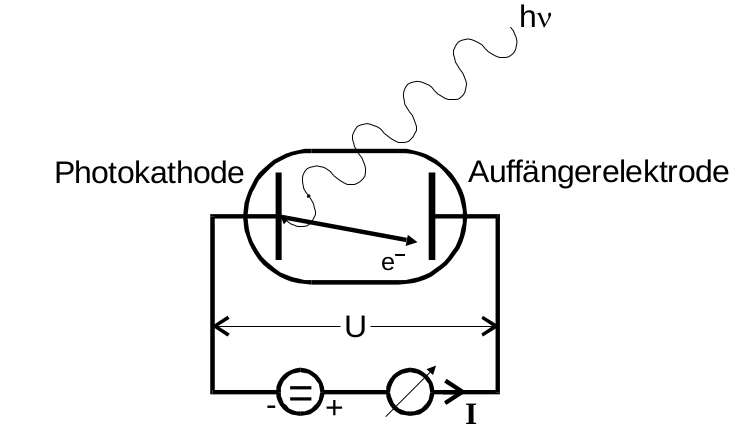
\includegraphics[height=5cm]{pictures/PrinzipielleAnordnung.png}
	\caption{Prinzipielle Anordnung zur Untersuchung des Photoeffektes
	\cite{anleitung}.}
	\label{fig:PrinzipielleAnordnung}
\end{figure}
Die experimentellen Ergebnisse lassen sich qualitativ zusammenfassen:
\begin{itemize}
	\item Der Fotostrom ist proportional zur Intensität der Lichtstrahlung.
	\item Die Energie eines einzelnen Photoelektrons ist proportional zur
		Lichtfrequenz und unabhängig von der Intensität.
	\item Unterhalb einer Grenzfrequenz tritt der Photoeffekt nicht auf.
\end{itemize}
Die Ergebnisse widersprechen den Erwartungen bei einem Wellencharakter: Unter der Annahme,
dass die Elektronen durch einfallende Photonen zu Schwingungen angeregt werden, würden
die Elektronen aus der Metallfläche heraustreten sobald die eigene Schwingungsamplitude groß
genug wäre. Dann müsste der Effekt aber auch  bei intensiver, langwelliger Strahlung
beobachtbar sein, was aber nach dem dritten Punkt nicht der Fall ist. Dadrüber hinaus
würden bei einem Wellenmodell bei bestimmte Frequenzen Resonanzphänomene auftreten und einen 
besonders starken Photoeffekt hervorrrufen, was im Experiment nicht beobachtet wird.

Die Beobachtungen lassen sich jedoch erklären, wenn man Licht nicht als gleichmäßige
Welle, sondern als diskrete Energiepakete (Photonen oder Lichtquanten) interpetiert.
Monochromatisches Licht sind in diesem Modell Photonen, die jeweils die Energie $h\nu$
besitzen und sich mit Lichtgeschwindigkeit gradlinig durch den Raum bewegen.
\\
Trifft das Photon auf ein Elektron in der Metalloberfläche, überträgt es seine Energie auf
das Elektron. Ein Teil der Energie wird als Austrittsarbeit $A_\text{k}$ dafür benötigt,
dass Elektron aus der Atom herauszubefördern, der Rest bleibt als kinetische Energie
erhalten. Die Energiegleichung lautet somit
\begin{equation}
	\label{eqn:theo:energiegleichung}
	h\nu = E_\text{kin} + A_\text{k}.
\end{equation}
Offensichtlich kann der Photoeffekt nur auftreten, wenn 
\begin{equation}
	h\nu > A_\text{k},
\end{equation}
wodurch sich auch die Grenzfrequenz erklären lässt. Außerdem folgt mit
\autoref{eqn:theo:energiegleichung} auch die Proportionalität zwischen Frequenz und
Elektronenenergie. Da in dem hier beschriebenen Modell das Photon mit genau einem Elektron
reagiert, ist auch der Zusammenhang zwischen Lichtintensität und Photostrom geklärt.


